\documentclass{article}
\usepackage{graphicx}
% \usepackage[export]{adjustbox}
\graphicspath{ {Images/} }
% \usepackage{babel,blindtext}



\author{Pseudo-Ku}
\title{Java Sudoku Solver using Backtracking}
\date{07 October 2020}

\begin{document}
    \begin{titlepage}
        \maketitle{}
    \end{titlepage}
    
    \tableofcontents

    % Aims
    \pagebreak 
    \section{Aims}
The main aim of this lab report is to review the performance of our group’s implementation of the Backtracking Algorithm on solving sudoku puzzles with varying amounts of zero spaces in the question puzzle. Conversely, one could also interpret it as reviewing the algorithm’s performance on solving sudoku puzzles with varying amounts of filled spaces or clues in the initial puzzle. In this report we hypothesize that the more open spaces (or the fewer number of clues) there are in the initial sudoku puzzle, then the more computation will be required to solve such a puzzle. 
\\\\
It is thus our goal to verify our theoretical assumptions (which will be expanded upon in subsequent sections) of the algorithm’s performance with the empirical evidence we obtain from running our program on many different sudoku puzzles. Simply put, we want to check that the algorithm has the same space and time complexities that we believe it to have theoretically. If this is not the case, then it is also our goal to determine why it is not. 
\\\\

    % Summary of Theory
    % \pagebreak 
    \section{Summary of Theory}
    
	Our initial assumption is that the Backtracking Algorithm will have the following space and time complexities when solving 9x9 sudoku puzzles:
	\\
	\subsection{Space Complexity : O($n^2$)}
	
	The initial and solved sudoku puzzle would need to be stored in a 2D matrix made up arrays of size n. Thus, in any case the space complexity would be O($n^2$).\cite{GeeksforGeeks}
	\\
	\subsection{Time complexity: O$(9^{n^2})$} 

There exists 9 possible options for every open space in the initial sudoku puzzle. In the worst case, the algorithm would need to visit every open space in every iteration of the algorithm and change all of the values 9 times. Thus, the time complexity in the worse case would be O$(9^{k^2})$ where k is the number of open spaces. In the best case, the algorithm would need to visit every open space once and change the value within that open space once. Thus, the time complexity in the best case would be O($n^2$). \cite{GeeksforGeeks}

	
	



    % Experimental Methodology
    \pagebreak 
    \section{Experimental Methodology}
    As stated in our aims, our initial assumption is that more open spaces (or fewer clues) in the initial sudoku puzzle will result in more computation needed in order to find the unique solution of a given puzzle. We have utilized 3 metrics to measure the performance of the algorithm, namely number of comparisons, number of changes, and the amount of time taken to return a unique solution to a given puzzle. Please see below discussions on our chosen metrics:

    \subsection{Number of comparisons}
    This metric measures the number of times the program compares the current value of the puzzle it is on with the rest of the incomplete puzzle. At each iteration, the program checks that the current value does not break the puzzle (ie: it checks to see that the current value of the puzzle is not repeated within that value’s row, column or sub-grid. It is our assumption that puzzles with more empty spaces will need more comparisons than puzzles with less empty spaces. \cite{{inproceedings}}

    \subsection{Number of changes}
    This metric measures the number of times the program changes a value it has just compared to a value that will not break the board (since it found that the value at the position is currently on has broken the board). It also measures the number of times the program changes an empty space to a filled space (a space with any positive integer less than 10).
    Again, our group assumes that the program will make more changes to puzzles with more empty spaces than it will to puzzles with less empty spaces. \cite{{inproceedings}}

    \subsection{Run Time}   
    This metric measures the length of time (in milliseconds) it takes for the program to output a unique solution to a given puzzle. It is our assumption that puzzles with more empty spaces will take much longer to complete than puzzles with less empty spaces. \cite{{inproceedings}}
\\\\
Initially, we had decided to use a puzzle’s difficulty, instead of the number of open spaces it has, as the independent variable to measure the performance of our program. We had graphed the difficulty of the graph against the number of comparisons, number of changes, and run time to solve the puzzle. However, this metric was abandoned for a number of reasons. Firstly, the graphs that were generated using this variable gave very little insight to the performance of our program (if any). Secondly, we found that in some cases puzzles of differing difficulties gave the same results. This is obviously incorrect, because an easy puzzle should not be getting the same results as a medium puzzle for example. We discovered that a ‘hard’ easy puzzle would yield the same results as an ‘easy’ medium puzzle. Thirdly, it is very difficult to define a puzzle’s difficulty. Difficulty is a concept that can be understood by a human, but it would be very abstract to a computer. One could look at the number of clues to determine that puzzle’s difficulty, but this is approach is a bit simplistic, as the positions of those clues could be a factor to consider when defining difficulty. 
\\\\
To measure the performance of our program we started off with the initial solved puzzle, ran our program on it and recorded and plotted the results. Then we randomly removed 3 clues from that puzzle and repeated that same process. This process was repeated until there were no more clues left in that puzzle (ie: the puzzle was left only with white spaces). This process made up our empirical experimentation. Here are some illustrations of the first three iterations of the algorithm of a puzzle taken from sudoku.com (2020) \cite{{Sudoku:2020}}
\\\\


\begin{figure}[!htb]
\minipage{0.32\textwidth}
  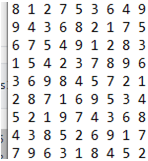
\includegraphics[width=\linewidth]{iteration1.png}
  \caption{Iteration 1}\label{fig:awesome_image1}
\endminipage\hfill
\minipage{0.32\textwidth}
  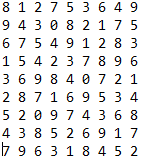
\includegraphics[width=\linewidth]{iteration2.png}
  \caption{Iteration 2}\label{fig:awesome_image2}
\endminipage\hfill
\minipage{0.32\textwidth}%
  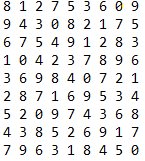
\includegraphics[width=\linewidth]{iteration3.png}
  \caption{Iteration 3}\label{fig:awesome_image3}
\endminipage
\end{figure}


As you can see, the puzzle in the first iteration has no white spaces as that is the solved puzzle. The puzzle in the second iteration has white spaces in positions (1,3), (4, 5) and (6,3). The puzzle in the third iteration has white spaces in positions (1,3), (4, 5), (6,3), (0,7), (3,1) and (8,8). Results of the performance of this implementation of the algorithm will be presented, interpreted and reviewed in subsequent sections.

    
    % Presentation of results
    \pagebreak 
    \section{Presentation of results}
    \begin{figure}[h]
        \centering
        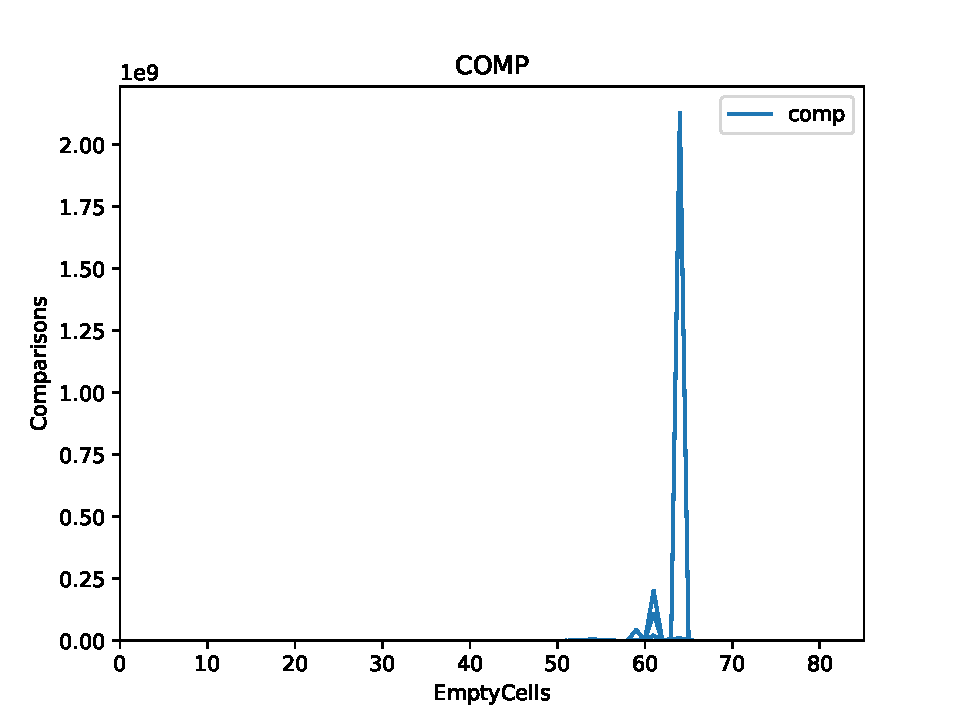
\includegraphics[width=1\textwidth]{COMP.pdf}
        \caption{Comparisons Plot}
    \end{figure}
        

    % Interpretation of results
    % \pagebreak 
    \section{Interpretation of results}

    % Theory relationship
    % \pagebreak 
    \section{Theory relationship}

    % Conclusion
    % \pagebreak 
    \section{Conclusion}

    % References
    \pagebreak
    \section{References}
    \bibliographystyle{plain}
    \bibliography{file.bib}

    % Acknowledgements
    % \pagebreak 
    \section{Acknowledgements}
\end{document}